% docs/slides/preamble.tex -- 五份 deck 共享
\documentclass[aspectratio=169,11pt]{beamer}

% ==== 中文与字体 ====
\usepackage[UTF8,fontset=none]{ctex}
\usepackage{fontspec}

\IfFontExistsTF{PingFang SC}{%
  \setCJKmainfont{PingFang SC}[BoldFont=PingFang SC,ItalicFont=PingFang SC,AutoFakeSlant=0.15]
  \setCJKsansfont{PingFang SC}[ItalicFont=PingFang SC,AutoFakeSlant=0.15]
  \setCJKmonofont{PingFang SC}
}{%
  \IfFontExistsTF{Source Han Sans SC}{%
    \setCJKmainfont{Source Han Sans SC}
    \setCJKsansfont{Source Han Sans SC}
  }{%
    \IfFontExistsTF{Noto Sans CJK SC}{%
      \setCJKmainfont{Noto Sans CJK SC}
      \setCJKsansfont{Noto Sans CJK SC}
    }{%
      \setCJKmainfont{Heiti SC}
      \setCJKsansfont{Heiti SC}
    }
  }
}

\IfFontExistsTF{Helvetica Neue}{\setmainfont{Helvetica Neue}}{%
  \IfFontExistsTF{Inter}{\setmainfont{Inter}}{}}
\IfFontExistsTF{JetBrains Mono}{\setmonofont{JetBrains Mono}[Scale=0.85]}%
  {\setmonofont{Menlo}[Scale=0.85]}

% ==== 颜色 ====
\usepackage{xcolor}
\definecolor{cMain}{HTML}{1F4E79}
\definecolor{cAccent}{HTML}{E07A1F}
\definecolor{cGray}{HTML}{595959}
\definecolor{cMute}{HTML}{F4F4F4}
\definecolor{cOK}{HTML}{2E7D32}
\definecolor{cBad}{HTML}{B23A3A}
\definecolor{cWarn}{HTML}{C8A300}

% ==== 主题 ====
\usepackage{tcolorbox}
\usetheme{metropolis}
\metroset{progressbar=frametitle,numbering=fraction,block=fill}
\setbeamercolor{frametitle}{bg=cMain,fg=white}
\setbeamercolor{progress bar}{fg=cAccent,bg=cMute}
\setbeamercolor{alerted text}{fg=cAccent}
\setbeamercolor{title}{fg=cMain}

% metropolis 默认尝试 Fira Sans，未安装时 fallback 到 Latin Modern Sans。
% 这里在主题加载后显式覆盖，强制使用 macOS 上一定存在的 Helvetica Neue，
% 跟中文 PingFang 风格一致；找不到则按顺序尝试 Inter / Arial。
\IfFontExistsTF{Helvetica Neue}{%
  \setsansfont{Helvetica Neue}%
}{%
  \IfFontExistsTF{Inter}{\setsansfont{Inter}}{%
    \IfFontExistsTF{Arial}{\setsansfont{Arial}}{}}%
}

% ==== TikZ ====
\usepackage{tikz}
\usetikzlibrary{positioning,arrows.meta,fit,shapes.geometric,calc,%
  decorations.pathmorphing,backgrounds}

\tikzset{
  node-box/.style={draw=cMain,thick,rounded corners=2pt,
    minimum height=8mm,minimum width=18mm,align=center,font=\small},
  node-state/.style={draw=cMain,thick,circle,minimum size=14mm,
    align=center,font=\small},
  node-ok/.style={draw=cOK,thick,fill=cOK!10},
  node-warn/.style={draw=cWarn,thick,fill=cWarn!15},
  node-bad/.style={draw=cBad,thick,fill=cBad!10},
  % 色盲友好的状态机三态：蓝 (正常/Closed) / 橙 (告警/Open) / 灰 (中间/HalfOpen)
  % 避免 red-green 二元区分，改用 hue + lightness 双通道。
  node-state-normal/.style={draw=cMain,thick,fill=cMain!12},
  node-state-alert/.style={draw=cAccent,thick,fill=cAccent!18},
  node-state-transition/.style={draw=cGray,thick,fill=cGray!18},
  arrow/.style={-{Stealth[length=2mm]},thick,draw=cMain},
  arrow-async/.style={-{Stealth[length=2mm]},thick,dashed,draw=cGray},
  arrow-bad/.style={-{Stealth[length=2mm]},thick,draw=cBad},
  arrow-alert/.style={-{Stealth[length=2mm]},thick,draw=cAccent},
  lifeline/.style={dashed,thick,draw=cGray},
}

% ==== 代码 ====
\usepackage{listings}
\lstdefinelanguage{Go}{
  morekeywords={break,case,chan,const,continue,default,defer,else,
    fallthrough,for,func,go,goto,if,import,interface,map,package,range,
    return,select,struct,switch,type,var,nil,true,false,iota},
  morekeywords=[2]{string,int,int64,uint,uint64,bool,byte,error,context},
  sensitive=true,
  morecomment=[l]//,morecomment=[s]{/*}{*/},
  morestring=[b]",morestring=[b]`,
}
\lstdefinelanguage{LuaRedis}{
  morekeywords={and,break,do,else,elseif,end,false,for,function,if,in,
    local,nil,not,or,repeat,return,then,true,until,while},
  morekeywords=[2]{redis,call,KEYS,ARGV,tonumber,HGET,HSET,GET,SET,
    DECR,DECRBY,INCR,INCRBY,EXPIRE,PEXPIRE,ZADD,ZCARD,ZREMRANGEBYSCORE,
    EVAL,EVALSHA},
  sensitive=true,
  morecomment=[l]{--},
  morestring=[b]",morestring=[b]',
}

\lstdefinestyle{base}{
  basicstyle=\ttfamily\scriptsize,
  numbers=left,numberstyle=\tiny\color{cGray},
  keywordstyle=\color{cMain}\bfseries,
  keywordstyle=[2]\color{cAccent},
  stringstyle=\color{cOK},
  commentstyle=\color{cGray}\itshape,
  backgroundcolor=\color{cMute},
  frame=single,framerule=0pt,
  showstringspaces=false,
  breaklines=true,
  tabsize=2,
  columns=fullflexible,
}
\lstset{style=base}

% ==== 三线表与附录页码 ====
\usepackage{booktabs}
\usepackage{appendixnumberbeamer}

% ==== 页脚来源标注 ====
\newcommand{\srcnote}[1]{{\color{cGray}\scriptsize\itshape #1}}

% 关键论点框
\newcommand{\keypoint}[1]{%
  \begin{tcolorbox}[colback=cMute,colframe=cMain,boxrule=0.5pt,arc=2pt]%
  #1\end{tcolorbox}}


\title{防超发与抢购库存}
\subtitle{Redis 原子扣减 vs \texttt{SELECT FOR UPDATE} 的实战对比}
\author{gomall · 后端实战}
\date{}

\begin{document}

\maketitle

\begin{frame}{今日大纲}
\tableofcontents
\end{frame}

% ============== 1. 故事 ==============
\section{超发的代价}

\begin{frame}{618 那一夜}
\begin{itemize}
  \item 配额：10 万张满 200 减 50 优惠券。
  \item 凌晨开抢，3 分钟全光，运营群一片欢呼。
  \item 财务次日对账发现：实际发出 23 万张。
\end{itemize}
\vspace{2mm}
\keypoint{超发 13 万 $\times$ 50 元 = 650 万。一行代码值半个 P0。}
\srcnote{源自 docs/blog/02-anti-oversell.md \S 优惠券超发能赔多少钱}
\end{frame}

\begin{frame}{check-then-act 的经典时序}
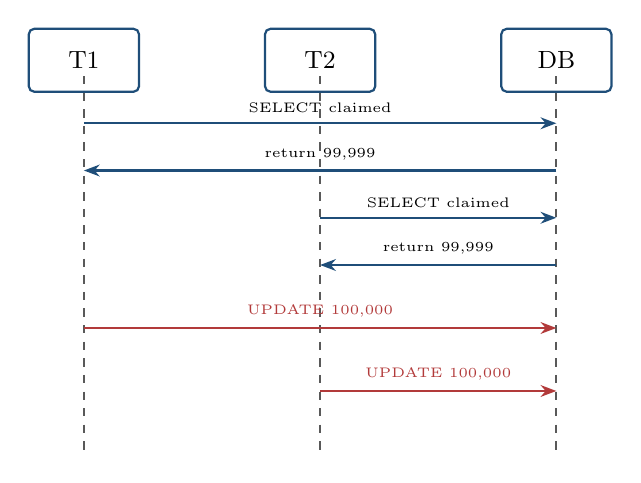
\begin{tikzpicture}[node distance=10mm]
  \foreach \name/\x in {T1/0, T2/30, DB/60} {
    \node[node-box,minimum width=14mm] at (\x mm,0) (\name) {\name};
    \draw[lifeline] (\x mm,-2mm) -- (\x mm,-50mm);
  }
  \draw[arrow] (0,-8mm) -- node[above,font=\tiny]{SELECT claimed} (60mm,-8mm);
  \draw[arrow] (60mm,-14mm) -- node[above,font=\tiny]{return 99{,}999} (0,-14mm);
  \draw[arrow] (30mm,-20mm) -- node[above,font=\tiny]{SELECT claimed} (60mm,-20mm);
  \draw[arrow] (60mm,-26mm) -- node[above,font=\tiny]{return 99{,}999} (30mm,-26mm);
  \draw[arrow-bad] (0,-34mm) -- node[above,font=\tiny\color{cBad}]{UPDATE 100{,}000} (60mm,-34mm);
  \draw[arrow-bad] (30mm,-42mm) -- node[above,font=\tiny\color{cBad}]{UPDATE 100{,}000} (60mm,-42mm);
\end{tikzpicture}
\vspace{1mm}
\small 两个事务都看到 99{,}999，都觉得"还能发一张" $\to$ 超发。
\end{frame}

\begin{frame}[fragile]{错法：单条 SQL 看似"原子"}
\begin{lstlisting}[language=SQL,basicstyle=\ttfamily\scriptsize]
UPDATE coupon_batch
   SET claimed = claimed + 1
 WHERE id = ? AND claimed < total;
\end{lstlisting}
\begin{itemize}
  \item 看起来一条原子 UPDATE，"行锁会兜底"。
  \item 但还要写 \texttt{user\_coupon} 记录、校验 per-user 配额 —— 多条 SQL 的原子性回到了零。
  \item 一旦套上事务，并发下还是要靠 row lock 串行化，吞吐塌方。
\end{itemize}
\srcnote{对应 docs/blog/02-anti-oversell.md \S 看起来天衣无缝}
\end{frame}

% ============== 2. 方案矩阵 ==============
\section{方案矩阵}

\begin{frame}{五种防超发方案}
\begin{tabular}{@{}lllll@{}}
\toprule
方案 & 一致性 & 吞吐 & 复杂度 & 适用 \\
\midrule
悲观锁 \texttt{FOR UPDATE} & 强 & 低 & 低 & 低频/账务 \\
乐观锁 \texttt{version} & 强 & 中 & 中 & 中频/CAS 友好 \\
Redis \texttt{DECR} 单命令 & 强 & 高 & 低 & 单一计数 \\
Redis Lua 多 key & 强 & 高 & 中 & \textbf{多条件抢资源} \\
Redlock 分布式锁 & 强 & 中 & 高 & 跨资源/慎用 \\
\bottomrule
\end{tabular}
\vspace{3mm}
\small 本项目实现了两种：\textbf{Redis Lua} (常用) 和 \texttt{FOR UPDATE} (对比基线)。
\srcnote{service/coupon.go:65--99 mode 切换}
\end{frame}

\begin{frame}{两种模式可热切换}
\begin{tikzpicture}[node distance=8mm and 16mm]
  \node[node-box] (cli) {Client};
  \node[node-box,right=of cli] (svc) {CouponSrv\\.Claim};
  \node[node-box,above right=of svc,node-warn] (db) {DB 悲观锁};
  \node[node-box,below right=of svc,node-ok] (rd) {Redis Lua};
  \node[node-box,right=of db] (mysql) {MySQL};
  \node[node-box,right=of rd] (redis) {Redis};
  \draw[arrow] (cli) -- (svc);
  \draw[arrow] (svc.east) -- node[above,font=\tiny]{mode=db} (db.west);
  \draw[arrow] (svc.east) -- node[below,font=\tiny]{mode=redis} (rd.west);
  \draw[arrow] (db) -- (mysql);
  \draw[arrow] (rd) -- (redis);
\end{tikzpicture}
\vspace{1mm}
\small 一行配置 \texttt{mode=db} 或 \texttt{mode=redis} 切换两套实现，便于压测对比。
\srcnote{service/coupon.go:65--99}
\end{frame}

% ============== 3. DB 锁 ==============
\section{DB 悲观锁}

\begin{frame}[fragile]{\texttt{SELECT FOR UPDATE} 加 count 校验}
\begin{lstlisting}[language=Go,firstnumber=41,
  caption={\srcnote{repository/db/dao/coupon.go:41--85}}]
err := d.Transaction(func(tx *gorm.DB) error {
    var batch model.CouponBatch
    if err := tx.Set("gorm:query_option", "FOR UPDATE").
        Where("id = ?", batchId).First(&batch).Error; err != nil { return err }
    if batch.Claimed >= batch.Total { return errors.New("已抢光") }
    var owned int64
    tx.Model(&model.UserCoupon{}).Where("user_id = ? AND batch_id = ?",
        userId, batchId).Count(&owned)
    if owned >= batch.PerUser { return errors.New("超出单人上限") }
    tx.Model(&model.CouponBatch{}).Where("id = ?", batch.ID).
        Update("claimed", gorm.Expr("claimed + 1"))
    return tx.Create(uc).Error
})
\end{lstlisting}
\end{frame}

\begin{frame}{DB 锁的原理：行锁串行化}
\begin{tikzpicture}[node distance=10mm]
  \foreach \name/\x in {T1/0, T2/30, T3/60, MySQL/90} {
    \node[node-box,minimum width=14mm] at (\x mm,0) (\name) {\name};
    \draw[lifeline] (\x mm,-2mm) -- (\x mm,-55mm);
  }
  \draw[arrow] (0,-8mm) -- node[above,font=\tiny]{FOR UPDATE} (90mm,-8mm);
  \node[font=\tiny,text=cOK] at (45mm,-14mm) {T1 拿到行锁，T2/T3 BLOCK};
  \draw[arrow] (0,-22mm) -- node[above,font=\tiny]{COMMIT} (90mm,-22mm);
  \draw[arrow] (30mm,-30mm) -- node[above,font=\tiny]{FOR UPDATE 解除阻塞} (90mm,-30mm);
  \draw[arrow] (30mm,-38mm) -- node[above,font=\tiny]{COMMIT} (90mm,-38mm);
  \draw[arrow] (60mm,-46mm) -- node[above,font=\tiny]{FOR UPDATE 解除阻塞} (90mm,-46mm);
\end{tikzpicture}
\vspace{1mm}
\small 正确性满分 —— 但 N 个并发就是 N 倍延迟，DB 单点就是上限。
\end{frame}

\begin{frame}{DB 锁的代价}
\begin{itemize}
  \item 正确性强：行锁让整个 batch 真正串行。
  \item 吞吐上限：实测 RPS 50{,}142，\textbf{max 延迟 453ms}（尾延迟暴雷）。
  \item 索引选错时会从行锁升级为间隙锁甚至表锁。
  \item DB 是单点，扩容代价高于 Redis。
\end{itemize}
\srcnote{stressTest/REPORT.md \S 6. 优惠券 Redis vs DB 锁}
\end{frame}

% ============== 4. Redis Lua ==============
\section{Redis Lua 双 key}

\begin{frame}{双 key 设计}
\begin{tikzpicture}[node distance=20mm]
  \node[node-box,minimum width=42mm,minimum height=18mm,node-ok]
    (stk) {\texttt{coupon:batch:\{id\}:stock}\\剩余库存};
  \node[node-box,minimum width=42mm,minimum height=18mm,node-warn,right=of stk]
    (usr) {\texttt{coupon:user:\{uid\}:batch:\{id\}}\\该用户已领次数};
  \draw[arrow] (stk) -- node[above,font=\tiny]{Lua 原子绑定} (usr);
\end{tikzpicture}
\vspace{2mm}
\begin{itemize}
  \item 一段 Lua 里同时检查"还有库存"+"用户没超额"。
  \item 任何一步失败都不会改另一边 —— 这是双 key 必须 Lua 的本质。
\end{itemize}
\srcnote{repository/cache/coupon.go:12--44}
\end{frame}

\begin{frame}[fragile]{抢券 Lua 完整脚本}
\begin{lstlisting}[language=LuaRedis,firstnumber=30,
  caption={\srcnote{repository/cache/coupon.go:30--44}}]
local stock = tonumber(redis.call('GET', KEYS[1]))
if stock == nil or stock <= 0 then
    return -1
end
local owned = tonumber(redis.call('GET', KEYS[2]))
if owned == nil then owned = 0 end
if owned >= tonumber(ARGV[1]) then
    return -2
end
redis.call('DECR', KEYS[1])
redis.call('INCR', KEYS[2])
redis.call('EXPIRE', KEYS[2], tonumber(ARGV[2]))
return 1
\end{lstlisting}
\vspace{1mm}
\small 返回 1 = 成功；$-1$ = 已抢光；$-2$ = 超出单人上限。
\end{frame}

\begin{frame}{为什么这能保证不超发}
\begin{itemize}
  \item Redis 是单线程：Lua 脚本被当作一条命令，期间不接受其他客户端的命令。
  \item \texttt{DECR} 是真正的原子计数器；不可能"两个客户端同时把库存从 1 减到 -1"。
  \item 多条 \texttt{redis.call} 一起原子化 —— 不需要 WATCH/MULTI。
\end{itemize}
\vspace{2mm}
\keypoint{并发性来自客户端并行；防超发的根基是 Redis 服务端串行。}
\end{frame}

\begin{frame}[fragile]{落库失败要回滚 Redis}
\begin{lstlisting}[language=Go,firstnumber=83,
  caption={\srcnote{service/coupon.go:83--98}}]
ok, err := cache.ClaimCouponAtomic(ctx, u.Id, batchId, batch.PerUser)
if err != nil { return nil, err }
if !ok { return nil, errors.New("领取失败") }

uc, err := dao.NewCouponDao(ctx).PersistClaim(u.Id, batchId, batch.ValidDays)
if err != nil {
    // 落库失败回滚 redis，避免库存幽灵消耗
    cache.RollbackCouponStock(ctx, u.Id, batchId)
    return nil, err
}
return uc, nil
\end{lstlisting}
\end{frame}

\begin{frame}{回滚也可能失败：定时对账兜底}
\begin{tikzpicture}[node distance=10mm and 16mm]
  \node[node-box,node-warn] (redis) {Redis 库存};
  \node[node-box,right=of redis] (db) {DB \texttt{user\_coupon}};
  \node[node-box,below right=8mm and 4mm of redis,node-bad] (ghost) {幽灵差额};
  \node[node-box,below=14mm of ghost] (job) {定时对账 job};
  \draw[arrow-async] (redis) -- (db);
  \draw[arrow-bad] (redis) -- (ghost);
  \draw[arrow-bad] (db) -- (ghost);
  \draw[arrow] (ghost) -- (job);
  \draw[arrow] (job) to[bend left=35] node[right,font=\tiny]{补/扣}(redis);
\end{tikzpicture}
\vspace{1mm}
\small "Redis 扣成功 + DB 写失败 + 回滚也失败" 是真实存在的低概率事件；定时对账是终极兜底。
\end{frame}

\begin{frame}[fragile]{单测：500 抢 100 零超发}
\begin{lstlisting}[language=Go,firstnumber=11,
  caption={\srcnote{repository/cache/coupon\_test.go:11--46}}]
const total = 100
const concurrency = 500
InitCouponStock(ctx, batchId, total, time.Minute)
var success int64; var wg sync.WaitGroup
for i := 1; i <= concurrency; i++ {
    wg.Add(1); uid := uint(i)
    go func() {
        defer wg.Done()
        ok, _ := ClaimCouponAtomic(ctx, uid, batchId, 1)
        if ok { atomic.AddInt64(&success, 1) }
    }()
}
wg.Wait()
if got := atomic.LoadInt64(&success); got != total {
    t.Fatalf("oversell or undersell: want %d, got %d", total, got)
}
\end{lstlisting}
\end{frame}

% ============== 5. 性能 ==============
\section{压测对比}

\begin{frame}{Redis Lua vs DB 锁：尾延迟差 3 倍}
\begin{tabular}{@{}lrrrr@{}}
\toprule
方案 & RPS & avg & p95 & \textbf{max} \\
\midrule
Redis Lua & 51{,}362 & 1.24ms & 3.52ms & \textbf{136ms} \\
DB 悲观锁 & 50{,}142 & 1.29ms & 3.65ms & \textbf{453ms} \\
\bottomrule
\end{tabular}
\vspace{3mm}
\srcnote{stressTest/REPORT.md \S 链路压测表 第 5/6 行 + \S 6}

\vspace{2mm}
\small RPS 接近：因为 PerUser=1 让单用户两边都被卡在 1 张。\\
关键差异在尾延迟：DB 的 \textbf{max 453ms} 暴露了行锁排队的真实成本。
\end{frame}

\begin{frame}{选型直觉}
\keypoint{抢资源类必须 Redis Lua；DB 锁只配低频高一致场景。}
\begin{itemize}
  \item 秒杀、抢券、限购：Redis Lua（毫秒级，可水平扩容）。
  \item 账务转账、对账冲销：DB 事务 + 行锁（最终落 DB，逻辑统一）。
  \item 跨多个资源：考虑 Saga（见 Deck 4），别堆 Redlock。
\end{itemize}
\end{frame}

% ============== 6. 进阶：下单库存 ==============
\section{进阶：双桶库存}

\begin{frame}{下单场景的 available / reserved}
\begin{tikzpicture}[node distance=28mm]
  \node[node-box,minimum width=32mm,minimum height=18mm,node-ok] (av)
    {available\\\texttt{stock:available:\{pid\}}};
  \node[node-box,minimum width=32mm,minimum height=18mm,node-warn,right=of av] (rv)
    {reserved\\\texttt{stock:reserved:\{pid\}}};
  \node[font=\scriptsize,below=12mm of av] (sold) {真正消耗 (支付成功)};

  \draw[arrow,bend left=18] (av) to node[above,font=\tiny]{reserve(n) Lua} (rv);
  \draw[arrow,bend left=18] (rv) to node[below,font=\tiny]{release(n) 取消/超时} (av);
  \draw[arrow] (rv) -- node[right,font=\tiny]{commit(n) 支付} ($(rv)+(0,-22mm)$);
\end{tikzpicture}
\srcnote{repository/cache/inventory.go:10--75}
\end{frame}

\begin{frame}[fragile]{reserve / commit / release 三脚本}
\begin{lstlisting}[language=Go,firstnumber=78,
  caption={\srcnote{repository/cache/inventory.go:78--125}}]
// 预扣: available -= n, reserved += n
func ReserveStock(ctx context.Context, productID uint, n int64) error

// 支付成功: reserved -= n
func CommitReservation(ctx context.Context, productID uint, n int64) error

// 取消/超时: reserved -= n, available += n
func ReleaseReservation(ctx context.Context, productID uint, n int64) error
\end{lstlisting}
\vspace{1mm}
\small 三段 Lua 守护一个不变量：\texttt{available + reserved + sold == 初始库存}。
\end{frame}

\begin{frame}{设计决策清单}
\begin{itemize}
  \item 库存源：DB 是真相之源，Redis 是高并发缓冲。
  \item PerUser 限制：用独立的 user 计数器，不要塞进库存 key。
  \item Redis 重启：用 RDB/AOF + 启动时从 DB 重灌。
  \item TTL 设到活动结束 + 24h，留出对账窗口。
  \item Lua 用 \texttt{NewScript} 缓存 SHA，避免每次都传完整脚本。
\end{itemize}
\end{frame}

% ============== Q&A ==============
\appendix

\begin{frame}{面试 Q\&A（上）}
\textbf{Q1}：100 张券，500 并发，怎么保证不超发？\\
\hspace{4mm}\small A：Lua 脚本一次性原子执行"check + DECR"，Redis 单线程做兜底。

\vspace{2mm}
\textbf{Q2}：Redis 扣成功但 DB 落库失败，怎么办？\\
\hspace{4mm}\small A：立即 \texttt{RollbackCouponStock} 回滚；万一回滚也失败靠定时对账兜底。

\vspace{2mm}
\textbf{Q3}：\texttt{SELECT FOR UPDATE} 用错索引会怎么样？\\
\hspace{4mm}\small A：走非唯一索引或全表扫，行锁可能升级成 GAP 锁甚至表锁，吞吐塌方。
\end{frame}

\begin{frame}{面试 Q\&A（下）}
\textbf{Q4}：为什么不能 \texttt{if stock>0 then DECR} 两条命令？\\
\hspace{4mm}\small A：客户端两次 RTT 之间会被插队，跟"先 GET 再 SET"一样竞态。

\vspace{2mm}
\textbf{Q5}：热点商品怎么分片库存？\\
\hspace{4mm}\small A：按 hash 分 N 个子桶，每个桶独立 DECR；空桶时漂到其他桶 (有序兜底)。

\vspace{2mm}
\textbf{反追问}：能用 Redlock 替代 Lua 吗？\\
\hspace{4mm}\small A：不该。Redlock 用来跨资源协调；单 key 抢资源用 Lua 又快又稳。
\end{frame}

\begin{frame}{代码位置一览}
\begin{description}
  \item[抢券 Lua]\srcnote{repository/cache/coupon.go:30--44}
  \item[DB 悲观锁]\srcnote{repository/db/dao/coupon.go:41--85}
  \item[mode 切换]\srcnote{service/coupon.go:65--99}
  \item[双桶库存]\srcnote{repository/cache/inventory.go:30--75}
  \item[500 并发单测]\srcnote{repository/cache/coupon\_test.go:11--46}
  \item[压测脚本]\srcnote{stressTest/coupon\_claim\_redis.js + coupon\_claim\_db.js}
\end{description}
\vspace{2mm}
\keypoint{复现：\texttt{k6 run stressTest/coupon\_claim\_redis.js}}
\end{frame}

\end{document}
